%%
%% Capítulo 4: Nurse: uma aplicação para produtividade em vacinações
%%

\mychapter{Nurse: uma aplicação para produtividade em vacinações}
\label{Cap:Implementacao}
Nessa seção, serão apresentadas os requisitos do sistema definidos e a arquitetura escolhida para a aplicação. Além disso, também serão apresentadas as telas do aplicativo, os possíveis fluxos de navegação e os principais pacotes utilizados para o desenvolvimento da aplicação Nurse.

O projeto foi desenvolvido utilizando a linguagem de programação Dart, com o framework Flutter. O seu repositório pode ser encontrado no \textit{GitHub}, em \url{https://github.com/Dojak220/nurse}. A documentação, que inclui a versão dessa monografia em formato \textit{pdf} e o seu respectivo projeto em \textit{LateX} também pode ser encontrada no \textit{Github}, em \url{https://github.com/Dojak220/nurse-docs}.
% [A fazer] Criar um GitHub Pages \url{https://dojak220.github.io/nurse/}.

\section{Arquitetura do Sistema}
\label{cap4:SubSec:ArquiteturaSistema}

\section{Telas}
\label{cap4:Sec:Telas}

\section{Pacotes e Bibliotecas}
\label{cap4:Sec:PacotesBibliotecas}

Nessa seção, serão apresentados os pacotes e bibliotecas utilizados no desenvolvimento do sistema. A tabela \ref{tab:packages} apresenta os pacotes utilizados no desenvolvimento do sistema e suas respectivas versões.

% [A fazer] Adicionar a tabela de pacotes e bibliotecas utilizados no sistema.
\begin{table}[]
  \begin{tabular}{|>{\raggedright\arraybackslash}m{0.28\textwidth}|m{0.17\textwidth}|m{0.45\textwidth}|}
    \hline
    \multicolumn{1}{|>{\centering\arraybackslash}m{23mm}|}{\textbf{Pacote}} 
    & \multicolumn{1}{>{\centering\arraybackslash}m{23mm}|}{\textbf{Versão}} 
    & \multicolumn{1}{>{\centering\arraybackslash}m{60mm}|}{\textbf{Descrição}}\\ \hline
    cupertino\_icons           & \^{} 0.17.0       & Repositório de ícones utilizados pelos \textit{widget}s do Cupertino \cite{cupertino-package}  \\ \hline
    sqflite\_sqlcipher         & \^{} 2.1.0        & Extensão ao \textit{sqflite} \cite{sqflite-package} que adiciona senha ao acesso o banco de dados \cite{sqlcipher-package} \\ \hline
    path                       & \^{} 1.8.0        & Biblioteca para manipulação de caminhos em multi-plataformas \cite{path-package}               \\ \hline
    provider                   & \^{} 6.0.3        & Encapsula o \textit{InheritedWidget}, tornando-o reutilizável e mais fácil de usar \cite{provider-package}\\ \hline
    flutter\_archive           & \^{} 5.0.0        & Biblioteca para criação e extração de arquivos ZIP \cite{flutter_archive-package}              \\ \hline
    flutter\_dotenv            & \^{} 5.0.2        & Carrega configurações para aplicação em tempo de execução \cite{flutter_dotenv-package}        \\ \hline
    flutter\_mobx              & \^{} 2.0.5        & Integração do MobX aos \textit{widget}s do \textit{Flutter}                                    \\ \hline
    mobx                       & \^{} 2.0.7        & Biblioteca para gerenciamento de estado na aplicação                                           \\ \hline
    syncfusion\_flutter\_xlsio & \^{} 20.2.50-beta & Pacote para criação de arquivos Excel (.xlsx) \cite{syncfusion_flutter_xlsio-package}          \\ \hline
    path\_provider             & \^{} 2.0.11       & \textit{Plugin} para encontrar locais no sistema em múltiplas plataformas \cite{path_provider-package}  \\ \hline
    open\_file                 & \^{} 3.2.1        & \textit{Plugin} para abertura de arquivos do sistema em múltiplas plataformas \cite{open_file-package} \\ \hline
    share\_plus:               & \^{} 4.4.0        & \textit{Plugin} para compartilhamento de arquivos a partir da aplicação \cite{share_plus-package}       \\ \hline
  \end{tabular}
  \caption{Pacotes utilizados no projeto}
  \label{tab:packages}
\end{table}


% [A revisar] nomes dos pacotes e bibliotecas 
Entre os pacotes e plugins utilizados, se destacam aqueles que estão relacionados com a persistência de dados (sqflite\_sqlcipher), com o gerenciamento de estado (mobx e flutter\_mobx), com a injeção de dependências (provider) e com a criação da planilha que será compartilhada (syncfusion\_flutter\_xlsio).

\subsection{\textit{Plugin}s \textit{sqflite\_sqlcipher} e \textit{sqflite}}
\label{cap4:Subsec:sqflite-sqlcipher-package}
O plugin \textit{sqflite} permite o uso do \textbf{SQLite} em aplicações \textit{Flutter} \cite{sqflite-package}. O \textit{sqflite\_sqlcipher}, por sua vez, adiciona ao primeiro a funcionalidade de criptografia do banco de dados através da biblioteca \textit{SQLCipher} \cite{sqlcipher-package}.

\subsection{Bibliotecas \textit{mobx} e \textit{flutter\_mobx}}
\label{cap4:Subsec:mobx-package}
O pacote \textit{mobx} é utilizado para a implementação do \textit{MobX} \ref{cap2:Subsec:MobX} nas aplicações em \textit{Dart/Flutter}. É com ele que o gerenciamento de estado segue o conceito de reatividade visto anteriormente, utilizando-se das suas principais classes: \textit{\textbf{Observable}}, responsável por criar o estado reativo da aplicação; e \textit{\textbf{Action}}, que definirá a função que muda esse estado. Além disso, para completar a tríade do MobX, este utiliza-se de um conjunto de reações, em forma de função, que são chamadas no momento em que o estado observado muda \cite{mobx-package}.

Em adição, têm-se o pacote \textit{flutter\_mobx}, o qual é responsável por implementar um \textit{widget} chamado \textit{\textbf{Observer}}. Este, por sua vez, garante que o seu \textit{widget} filho seja atualizado sempre que o estado relacionado a ele mude. O \textit{Observer} também é um representante das reações do MobX que, nesse caso, reage atualizando a interface do usuário \cite{flutter-mobx-package}.

No desenvolvimento da classe \textbf{HomeController}, a qual gerencia o estado observado pelos componentes da página \textbf{Home}, utilizou-se as classes \textbf{Action}, para definir a função responsável por alterar o estado observável, e \textbf{ObservableList}, uma variante da classe \textbf{Observable} para listas.

\begin{lstlisting}[caption={Uso do \textit{MobX} na classe \textbf{HomeController}}, label={lst:home_controller_mobx}]
  class HomeController {
    final ApplicationRepository applicationRepository;

    final applications = ObservableList<Application>.of(
      List<Application>.empty(growable: true),
    );

    late final fetchApplications = Action(getApplications);

    HomeController() : applicationRepository = DatabaseApplicationRepository() {
      fetchApplications();
    }

    Future<List<Application>> getApplications() async {
      final result = await applicationRepository.getApplications();
      applications.clear();
      applications.addAll(result.reversed);

      return applications;
    }

    /*...*/
  }
\end{lstlisting}

A propriedade \textit{applications} recebe, inicialmente, um \textbf{ObservableList} vazio do tipo \textit{Application} e a função \textit{fetchApplications} foi definida como a ação que modifica o estado observável, isto é, a lista de aplicações. A ação é chamada no construtor da classe \textbf{HomeController} para que a lista de aplicações seja preenchida assim que a classe for instanciada. Essa lista, por sua vez, é preenchida quando a busca realizada pela classe \textbf{ApplicationRepository} no banco de dados finaliza com sucesso.  A função \textit{fetchApplications} é chamada, também, toda vez que o usuário finaliza um novo cadastro de aplicação de vacina e é redirecionado novamente à tela inicial \textbf{Home}.

\begin{lstlisting}[caption={Uso do \textit{MobX} no \textit{widget} \textbf{Home}}, label={lst:home_page_mobx}]
  class Home extends StatelessWidget {
    /*...*/

    @override
    Widget build(BuildContext context) {
      return Scaffold(
        
        /*...*/
      
        floatingActionButton: VaccinationButton(
          newPage: "/vaccinations/new",
          onCallback: () => context.read<HomeController>().
          fetchApplications(),
        ),
        
        /*...*/

      );
    }
  }
\end{lstlisting}

No código que define a classe \textbf{Home}, mostrada parcialmente no trecho de código \ref{lst:home_page_mobx}, têm-se o \textit{widget} \textbf{Scaffold}, o qual possui a propriedade \textbf{\textit{floatingActionButton}}, que recebe o \textit{widget} \textbf{VaccinationButton}. A sua propriedade \textit{onCallback} recebe uma função que chama \textit{fetchApplications} da classe \textbf{HomeController}, para que a lista de aplicações seja atualizada. A forma como o estado é injetado na classe \textbf{Home} é explicado adiante, na \ref{cap4:Subsec:Provider}.

\subsection{Pacote \textit{provider}}
\label{cap4:Subsec:Provider}
Como descrito anteriormente, na \ref{cap2:Subsec:Provider}, o estado pode ser injetado em qualquer \textit{widget} por meio do \textit{Provider}. Sendo assim, utilizou-se o \textit{Provider} nesse projeto não para gerenciamento do estado diretamente, mas para injetar o estado gerenciado pelo \textit{mobx} em qualquer \textit{widget} da aplicação. Para isso, foi utilizado o pacote \textit{provider} \cite{provider-package}.

Desse pacote, utilizou-se duas estratégias principais:
\begin{itemize}
  \item \textbf{Provider.of<T>(context)}: injeta a classe T a partir do contexto passado via parâmetro. O Provider, então, busca na árvore de \textit{widgets} acima do \textit{widget} atual a instância mais próxima da classe T \cite{provider-package}. A seguir, no trecho de código \ref{lst:appliers_page_provider}, tem-se um exemplo de uso dessa estratégia.
  \item \textbf{context.read<T>().fn()}: assim como o anterior, utiliza-se do contexto para buscar a classe T desejada e, em seguida, faz uma chamada da função denominada \textit{fn} no exemplo, mas não passa a observar as mudanças de estado que ocorrem nessa classe, diferentemente da função \textit{watch} \cite{provider-package}. Um exemplo do seu uso foi apresentado no trecho de código \ref{lst:home_page_mobx}, no qual \textit{fetchApplications} representa a função \textit{fn} aqui descrita.
\end{itemize}

\begin{lstlisting}[caption={Uso do \textit{Provider} no \textit{widget} \textbf{Appliers}}, label={lst:appliers_page_provider}]
  class Appliers extends StatelessWidget {
    const Appliers({Key? key}) : super(key: key);

    @override
    Widget build(BuildContext context) {
      final controller = Provider.of<AppliersPageController>(context);
      /*...*/

      return EntityList<Applier>(
        title: "Aplicantes",
        controller: controller,
        /*...*/
      );
    }
  }
\end{lstlisting}

\subsection{Biblioteca Excel (XlsIO)}
\label{cap4:Subsec:syncfusion_flutter_xlsio}
Utilizando-se do pacote \textit{syncfusion\_flutter\_xlsio}, foi possível gerar um arquivo \textit{.xlsx} a partir de uma lista de aplicações de vacina. Para isso, criou-se uma classe chamada \textbf{ExcelService} que possui dois métodos públicos: \textbf{\textit{shareExcelFile}} e \textbf{\textit{openExcelFile}}. Cada um desses métodos é chamado quando o usuário segue o fluxo apresentado na figura \ref{fig:fluxo_exportar_dados} e descrito em detalhes na seção \ref{cap5:SubSec:FluxoExportacao}.

O método \textbf{\textit{shareExcelFile}} cria um arquivo \textit{.xlsx} e permite que o usuário o compartilhe, enquanto o método \textbf{\textit{openExcelFile}} cria um arquivo \textit{.xlsx} e o abre no aplicativo de planilhas do usuário. A seguir, na figura \ref{fig:excel_service_diagram}, tem-se o fluxo de execução de ambos os métodos dentro da classe \textbf{ExcelService}.

\begin{figure}[!ht]
  \centering
  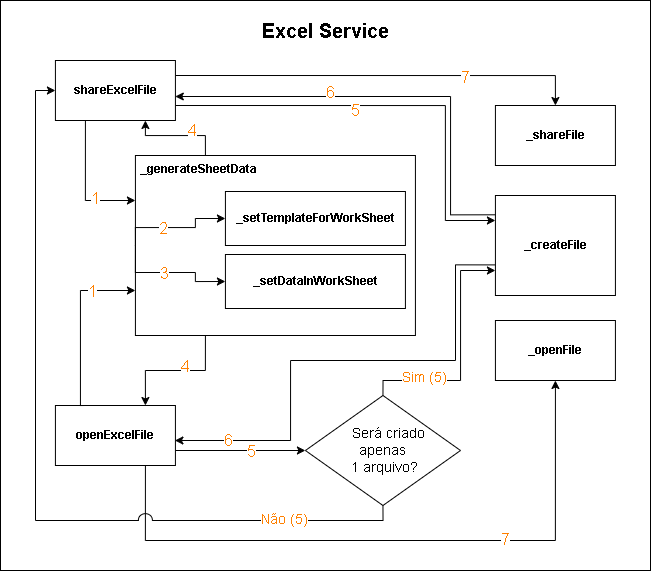
\includegraphics[width=\textwidth]{figuras/cap4/4_3_4_excel_service_diagram.png}
  \caption{Descritivo de fluxo dos métodos da classe \textbf{ExcelService}}
  \label{fig:excel_service_diagram}
\end{figure}

A ordem de execução dos métodos segue a ordem das setas numeradas. Cada um dos métodos é descrito a seguir:

\begin{itemize}
  \item \textbf{Etapa 1}: os métodos \textbf{\textit{shareExcelFile}} e \textbf{\textit{openExcelFile}} recebem como parâmetros a lista das aplicações cadastradas e o período de tempo que o usuário deseja exportar ou visualizar. Estas informações são, então, organizadas em um mapa de datas e aplicações e enviadas ao método \textbf{\textit{\_generateSheetData}}
  \item Etapas \textbf{2} e \textbf{3}: o método \textbf{\textit{\_generateSheetData}} recebe como parâmetro o mapa de datas e aplicações. A partir dos métodos \textbf{\textit{\_setTemplateForWorkSheet}} e \textbf{\textit{\_setDataInWorkSheet}}, um objeto do tipo \textbf{\textit{Workbook}} é, respectivamente estruturado e preenchido com os dados recebidos. Esse \textbf{\textit{Workbook}} é, então transformado em uma lista de bytes por meio de seu método interno \textbf{\textit{Workbook.saveAsStream()}}. Por fim, cada agrupamento de bytes é retornado em um novo mapa, onde a chave é a data das aplicações e o valor é um outro mapa de doses aplicadas e agrupamento de bytes.
  % [A fazer] Explicar na introdução porque essas planilhas devem ser separadas por data e dose
  \item \textbf{Etapa 4}: o método \textbf{\textit{\_generateSheetData}} retorna o agrupamento de bytes para as funções \textbf{\textit{shareExcelFile}} ou \textbf{\textit{openExcelFile}}, a depender de qual fluxo está sendo executado, e cada um desses agrupamentos será processado individualmente, como se segue.
  \item \textbf{Etapa 5}: para o método \textbf{\textit{openExcelFile}}, será verificado a quantidades de agrupamentos retornados. Caso seja apenas um, o arquivo será criado a partir desse agrupamento e passará ao próximo passo. Caso contrário, o fluxo desse método será finalizado e os dados serão redirecionados ao método \textbf{\textit{shareExcelFile}}. Já para este último, o fluxo é direto e cada cada conjunto de bytes separados por datas de aplicação e doses aplicadas será salvo em um arquivo.
  \item \textbf{Etapa 6}: considerando que o fluxo dos métodos \textbf{\textit{shareExcelFile}} e \textbf{\textit{openExcelFile}} foi o mesmo, ou seja, a criação dos arquivos na função \textbf{\textit{\_createFile}}, o(s) arquivo(s) recebido(s) será(ão) enviados de volta para as funções principais.
  \item \textbf{Etapa 7}: Por fim, o método \textbf{\textit{shareExcelFile}} chama a função \textbf{\textit{\_shareFile}} para compartilhar o arquivo gerado, enquanto o método \textbf{\textit{openExcelFile}} chama a função \textbf{\textit{\_openFile}} para abrir o arquivo gerado. Ambas as funções são descritas a seguir.
\end{itemize}

A função \textbf{\textit{\_shareFile}} recebe como parâmetro o arquivo gerado e, a partir da biblioteca \textit{share\_plus} e do seu método \textbf{\textit{Share.shareFiles}}, permite que o usuário compartilhe o arquivo gerado \cite{share_plus-package}. A função \textbf{\textit{\_openFile}}, por sua vez, também recebe o arquivo gerado de forma análoga à primeira função e, a partir da biblioteca \textit{open\_file} e do seu método \textbf{\textit{OpenFile.open}}, realiza a chamada a uma aplicação que possa abrir um arquivo no formato \textit{.xlsx}.

\section{Persistência de Dados}
\label{cap4:Sec:PersistenciaDados}
A persistência de dados, como descrita na seção \ref{cap2:Sec:PersistenciaDados}, é realizada por meio de um banco de dados relacional, o \textit{SQLite}. A biblioteca \textit{sqflite} é utilizada para a comunicação com o banco de dados \cite{sqflite-package}. A estrutura do banco de dados da aplicação como ela foi implementada é descrita nesta seção.

\subsection{Diagrama de Classes}
\label{cap4:SubSec:DiagramaClasses}
% ref. Cap 4 do livro Projeto de Banco de Dados Heuser
Foram definidas 9 entidades (ou classes) para a aplicação \textbf{Nurse}, as quais foram agrupadas em 3 macro-grupos: \textbf{Paciente}, \textbf{Vacinação} e \textbf{Infraestrutura}. Cada uma dessas entidades possui um identificador único, chamada chave primária (do inglês, \textit{Primary Key} (PK)) e algumas delas possuem uma ou mais chaves estrangeiras (do inglês, \textit{Foreign Key} (FK)) \cite{heuser09banco}. Além disso, cada entidade possui um ou mais atributos, que são apresentados na figura \ref{fig:diagrama_classes} e descritos a seguir.

\begin{figure}[!ht]
  \centering
  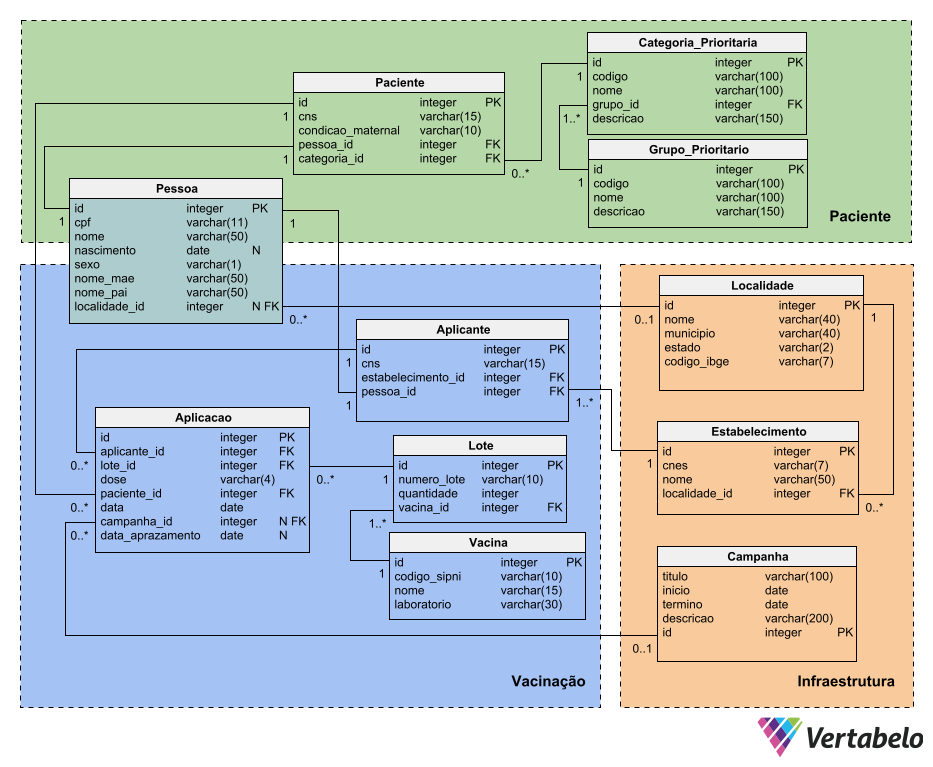
\includegraphics[width=\textwidth]{figuras/cap4/4_4_1_diagrama_classes.png}
  \caption{Diagrama de classe para a aplicação \textbf{Nurse}}
  \label{fig:diagrama_classes}
\end{figure}

\begin{itemize}
  \item \textbf{Pessoa}: é a entidade que representa uma pessoa, seja ela um paciente ou um profissional de saúde. Essa entidade possui os atributos \textbf{nome}, \textbf{cpf}, \textbf{data de nascimento}, \textbf{sexo}, \textbf{nome da mãe}, \textbf{nome do pai} e \textbf{localidade} onde reside. Essa entidade faz parte de dois grupo distintos: grupo 'Paciente' e grupo 'Aplicação', pois ela pode estar associada a um paciente ou a um aplicante da vacina.
  \item Grupo \textbf{Paciente}
  \begin{itemize}
    \item \textbf{Paciente}: é a entidade que representa um paciente. Essa entidade possui os atributos \textbf{cns} (número do Cartão Nacional de Saúde) e \textbf{condição maternal}. Além disso, a entidade \textbf{Paciente} possui duas chaves estrangeiras para as entidades \textbf{Pessoa} e \textbf{Categoria Prioritária}.
    \item \textbf{Categoria Prioritária}: é a entidade que representa uma categoria prioritária do paciente. Essa entidade possui os atributos \textbf{nome}, \textbf{código} e \textbf{descrição}. Além disso, a entidade \textbf{Categoria Prioritária} possui uma chave estrangeira para o seu \textbf{Grupo Prioritário}.
    \item \textbf{Grupo Prioritário}: é a entidade que representa um conjunto de categorias prioritárias. Um exemplo de grupo é 'Faixa Etária' e as categorias desse grupo são subconjuntos de idades (pessoas com mais de 60 anos, pessoas com menos de 18 anos etc...). Essa entidade possui os atributos \textbf{nome}, \textbf{código} e \textbf{descrição}.
  \end{itemize}
  \item Grupo \textbf{Infraestrutura}
  \begin{itemize}
    \item \textbf{Localidade}: é a entidade que representa uma localidade, seja ela uma comunidade ou uma cidade. Essa entidade possui os atributos \textbf{nome da localidade}, \textbf{município}, \textbf{estado} e \textbf{código do IBGE}.
    \item \textbf{Estabelecimento}: é a entidade que representa um estabelecimento de saúde. Essa entidade possui os atributos \textbf{nome} e \textbf{CNES} (Cadastro Nacional de Estabelecimentos de Saúde). Além disso, a entidade \textbf{Estabelecimento} possui uma chave estrangeira para a entidade \textbf{Localidade}.
    \item \textbf{Campanha}: é a entidade que representa uma campanha de vacinação. Essa entidade possui os atributos \textbf{título}, datas de \textbf{início} e \textbf{término} da campanha e sua \textbf{descrição}.
    % ref da sigla CNES: https://cnes.datasus.gov.br/ 21/11/2022 
  \end{itemize}
  \item Grupo \textbf{Vacinação}
  \begin{itemize}
    \item \textbf{Aplicante}: é a entidade que representa o profissional de saúde que realizou a aplicação da vacina no paciente. Essa entidade possui o atributo \textbf{cns}, assim como o paciente. Além disso, a entidade \textbf{Aplicante} possui duas chaves estrangeiras para as entidades \textbf{Pessoa} e \textbf{Estabelecimento}.
    \item \textbf{Vacina}: é a entidade que representa o agente imunizante que será aplicado no paciente. Essa entidade possui os atributos \textbf{nome} da vacina, seu \textbf{código SI-PNI} e o \textbf{laboratório} do fabricante.
    \item \textbf{Lote}: é a entidade que representa um lote de vacinas. Essa entidade possui os atributos \textbf{número do lote} e \textbf{quantidade de vacinas} no lote. Além disso, a entidade \textbf{Lote} possui uma chave estrangeira para a entidade \textbf{Vacina}.
    \item \textbf{Vacinação}: é a entidade central da aplicação. Ela representa todo o conjunto de informações que estão associadas ao ato de vacinar. Seus atributos representam essa centralidade. São eles: \textbf{Aplicante}, \textbf{Lote da vacina}, \textbf{Paciente} e \textbf{Campanha de vacinação}, as quais são todas chaves estrangeiras para outras tabelas. Além disso, a entidade \textbf{Vacinação} possui os atributos \textbf{dose da vacina}, \textbf{data de aplicação} e \textbf{data prazo} para próxima aplicação.
  \end{itemize}
\end{itemize}

Alguns desses atributos são obrigatórios, como o \textbf{cpf} e o \textbf{nome}, já outros podem ser deixados nulos, como é o caso do campo \textbf{sexo}, todos da tabela \textbf{Pessoa}. Além dessa, a tabela \textbf{Aplicação} também possui dois atributos chamados anuláveis, que são o identificador da tabela \textbf{Campanha} e o atributo \textbf{data de aprazamento}.

\subsection{Uso do Banco de Dados}
\label{cap4:Sec:UsoBancoDados}
















% \begin{algorithm}
% %% \SetLine
% \Entrada{$x$: vetores de valores; $y$ = $L(x)$; $p$: valor de entrada a ser calculado }
% \Saida{$s$ = $L(p)$}
% $n \leftarrow \mathtt{comprimento}(x)$\;
% $s \leftarrow 0$\;
% \Para {$i=1$ \Ate $n$} {
% 	$L \leftarrow 1$\;
% 	\Para {$j=1:1:n$} {
% 		\Se{$i \neq j$} {
% 			$L \leftarrow L* \left( \dfrac{p-x[j]}{x[i]-x[j]} \right) $
% 		}
% 	}
% 	$s \leftarrow s + L*y[i]$\;
% }
% \Retorna $s$\;
% \caption{Algoritmo para interpolação de Lagrange.}
% \label{algo:1}
% \end{algorithm}

% \begin{algorithm}
% %% \SetLine
% \Entrada{$a$: valor inicial; $b$: valor final; $n$: número de subintervalos (deve ser múltiplo de 2)  }
% \tcc{A função a ser integrada é definida em uma função denominada \texttt{f}, fora do escopo deste algoritmo.}
% \Saida{$I$ = integral de \texttt{f} entre $a$ e $b$}
% $h \leftarrow$ $\dfrac{b-a}{n}$\;
% $x[1] \leftarrow a$\;
% $y[1] \leftarrow f(a)$\;
% $I \leftarrow 0$\;
% $k \leftarrow 2$\;
% \Enqto {$k <= n$} {
% 	$x[i] \leftarrow x[i-1] + h$\;
% 	$y[i] \leftarrow f(x[i])$\;
% 	\eSe{$i \% 2 = 0$} {
% 		$I \leftarrow I + 4*y[i]$\;
% 	}
% 	{
% 		$I \leftarrow I + 2*y[i]$\;
% 	}
% 	$k = k+1$\;
% }
% $x[n+1] \leftarrow b$\;
% $y[n+1] \leftarrow f(x[i+1])$\;
% $I \leftarrow I + \dfrac{h}{3}*(I + y[n+1])$\;
% \Retorna $I$\;
% \caption{Algoritmo para a integração pelo primeiro método de Simpson.}
% \label{algo:2}
% \end{algorithm}
